\chapter{A Number Cannot Tell You What Rich Means}

Kenn Ricci has spent his working life around aircraft, a business in which a
small error can carry a large consequence. When James Dumoulin meets him at a
Beverly Hills event, Ricci does not answer the question about financial freedom
with the story of an aircraft, a company, or a deal. He gives a ratio.

His version is twenty-five times annual spending. A person who needs one unit a
year to sustain a chosen life, he says, is rich when twenty-five such units have
been accumulated. Someone who has built a ten-million-dollar annual lifestyle
would require two hundred and fifty million dollars under the same heuristic.
The point is not the multiplier. The point is that a fortune cannot be judged
without the life drawing upon it.

That reversal is easy to miss. Public talk about wealth usually begins with the
asset side: the salary, valuation, house, portfolio, or sale. Ricci begins with
the claim the life makes on those assets. Two people can own the same amount and
possess radically different degrees of freedom because they have different
obligations, expectations, health needs, dependents, and appetites for risk.

The first serious question about wealth is therefore not \emph{How much do you
have?} It is \emph{What must the money continue to do?}

\section{A balance has a job}

Let $S$ denote the annual spending required for a particular life. Let $q$
denote the fraction of an invested portfolio that the owner plans to draw in
the first year. The simplest planning identity is

\begin{equation}
P = \frac{S}{q},
\end{equation}

where $P$ is the capital required to support that draw before tax, fees, and
unplanned demands. Setting $q=0.04$ produces Ricci's ratio,

\begin{equation}
P = 25S.
\end{equation}

This is arithmetic, not a promise. A real plan has to survive inflation,
volatile returns, sequence risk, tax, fees, longevity, illness, dependents, and
changes in spending. Some assets cannot be sold gradually. Some income is
temporary. A person retiring young may need the capital to last far longer
than the historical period behind a familiar rule of thumb. A person with a
pension, flexible work, or reliably lower future costs may not ask the portfolio
to do the whole job.

Still, the identity performs useful work because it translates spectacle into
an obligation. Ten million dollars can be enormous as emergency protection,
insufficient to sustain a ten-million-dollar annual burn, and more than enough
for a household whose desired life costs a small fraction of that. The number
has not changed. Its assignment has.

Grant Cardone makes the same point in a harsher register. During a long
interview, he calls a million dollars inadequate and divides it over a person's
remaining years. The provocation is deliberately insensitive to what a million
dollars would mean to most households. Used carefully, however, the underlying
move is sound: convert the stock into the flow it must support.

Suppose a person has investable capital $P$, expects no further earned income,
and intends to spread principal evenly across $H$ years while ignoring returns,
inflation, and tax. The crude annual amount is

\begin{equation}
A = \frac{P}{H}.
\end{equation}

The calculation is too simple to be a retirement plan. It is useful as a
deflation device. A seven-figure headline becomes an annual capacity. A house
becomes shelter plus maintenance, tax, insurance, and illiquidity. A company
valuation becomes a contingent claim that may never convert at the quoted
price. The reader can finally ask whether the asset and the intended life fit.

Cardone's own childhood story adds the part that his provocation can obscure.
His father died while the family still depended on the father's income. The
loss was personal first, but it also revealed a structural financial fact: the
household had an income producer, not an income system that could continue
without him. Wealth, in this sense, includes the capacity of care and provision
to survive the temporary or permanent absence of the person doing the work.

This is why income and wealth must remain separate. Income is a flow arriving
under present conditions. Wealth is a stock of useful claims, capabilities, and
relationships that can continue to support choices when conditions change. The
flow can build the stock, but a large flow consumed entirely by a large life
leaves little behind.

\section{Security comes before spectacle}

Glenn Boyd answers the happiness question from the opposite end of the wealth
scale. School of Hard Knocks introduces him through a company transaction
described as exceeding a billion dollars. That figure belongs to the corporate
transaction; it should not be mistaken for a personal deposit. Boyd's answer
does not require us to know his final proceeds.

He begins with poverty. As a child, he says, he roofed houses in the Texas heat
with his father and later washed dishes with his mother. Money made a profound
difference when it ended that kind of insecurity. Bills could be paid. The
future contained room. Only after granting that material truth does he say that
more money stopped buying more happiness in the same way. The beach did not
become endlessly better. Luxury reached a point of repetition.

The economic intuition is diminishing marginal utility. If $C$ represents
consumption available to meet material needs, a simple model writes wellbeing
from consumption as $u(C)$, with

\begin{equation}
u'(C) > 0, \qquad u''(C) < 0.
\end{equation}

The first condition says that additional resources can improve life. The second
says that each additional unit may add less than the one before it. The model
does not locate a universal threshold. A dollar that buys food, medicine,
heating, safe housing, childcare, or escape from abusive work can have enormous
human value. A dollar that upgrades an already excellent hotel room may add
almost none. The same household can move between these regions when health,
family, or employment changes.

This gives us a more useful ladder than poor, middle class, rich, and wealthy:

\begin{enumerate}
\item \textbf{Survival.} Current necessities are uncertain. A disruption
  immediately threatens food, shelter, health, or safety.
\item \textbf{Stability.} Ordinary bills can be paid and a modest shock can be
  absorbed without destructive debt or dependence.
\item \textbf{Choice.} The household can refuse some bad work, move, learn,
  care for someone, or attempt a bounded experiment.
\item \textbf{Independence.} Chosen work and invested claims can support the
  desired life without compulsory labor on someone else's terms.
\item \textbf{Stewardship.} Surplus power is directed toward people, institutions,
  and futures beyond the owner's consumption.
\end{enumerate}

The boundaries are porous. Independence in one country may become instability
in another. A healthy single person and a household managing chronic illness
face different claims. Care work can reduce market income while increasing the
real wealth of a family. The ladder describes capabilities, not social worth.

A richer life needs three related goods that should not be collapsed into one.
\textbf{Abundance} is not luxury or display. It is having sufficient resources,
capabilities, relationships, time, and options to meet life with room rather
than constant scarcity. \textbf{Fulfillment} is the experience of using those
capacities for work, care, craft, service, love, or inquiry that feels worth the
effort it asks. \textbf{Contentment} is the freedom to recognize what is
sufficient and inhabit it, instead of allowing every comparison to reopen the
question.

These goods do not form a ladder. A person can be materially abundant and
unfulfilled, fulfilled by meaningful work while financially fragile, or
content with little while still lacking healthcare or safe housing. Nor is
contentment passivity. One can appreciate a life and still repair an injustice,
build a company, master a craft, or provide more securely for other people.
The test is whether further effort has a purpose beyond the discomfort of not
having more.

Financial freedom creates room for all three. It can secure resources and
options, release time for worthwhile commitments, and weaken the pressure to
keep accumulating merely because accumulation has become familiar. It cannot
guarantee any of them. Money can widen the feasible life; judgment, practice,
and relationship determine what occupies it.

This distinction explains why arguments about whether money buys happiness so
often fail.
One speaker remembers what money did near survival. Another describes what it
failed to do after abundance. Both can be telling the truth about different
regions of the same curve.

\section{The part of wealth that cannot compound}

Near the end of a retrospective interview, Tony Stephens holds a long strip of
paper in front of the camera. He treats it as a life from one to one hundred,
tears away the years beyond an illustrative life expectancy, then tears again
at his current age. The small portion left in his hand represents what might
remain. Illness, he adds, can change the quality of even that piece.

\begin{figure}[htbp]
\centering
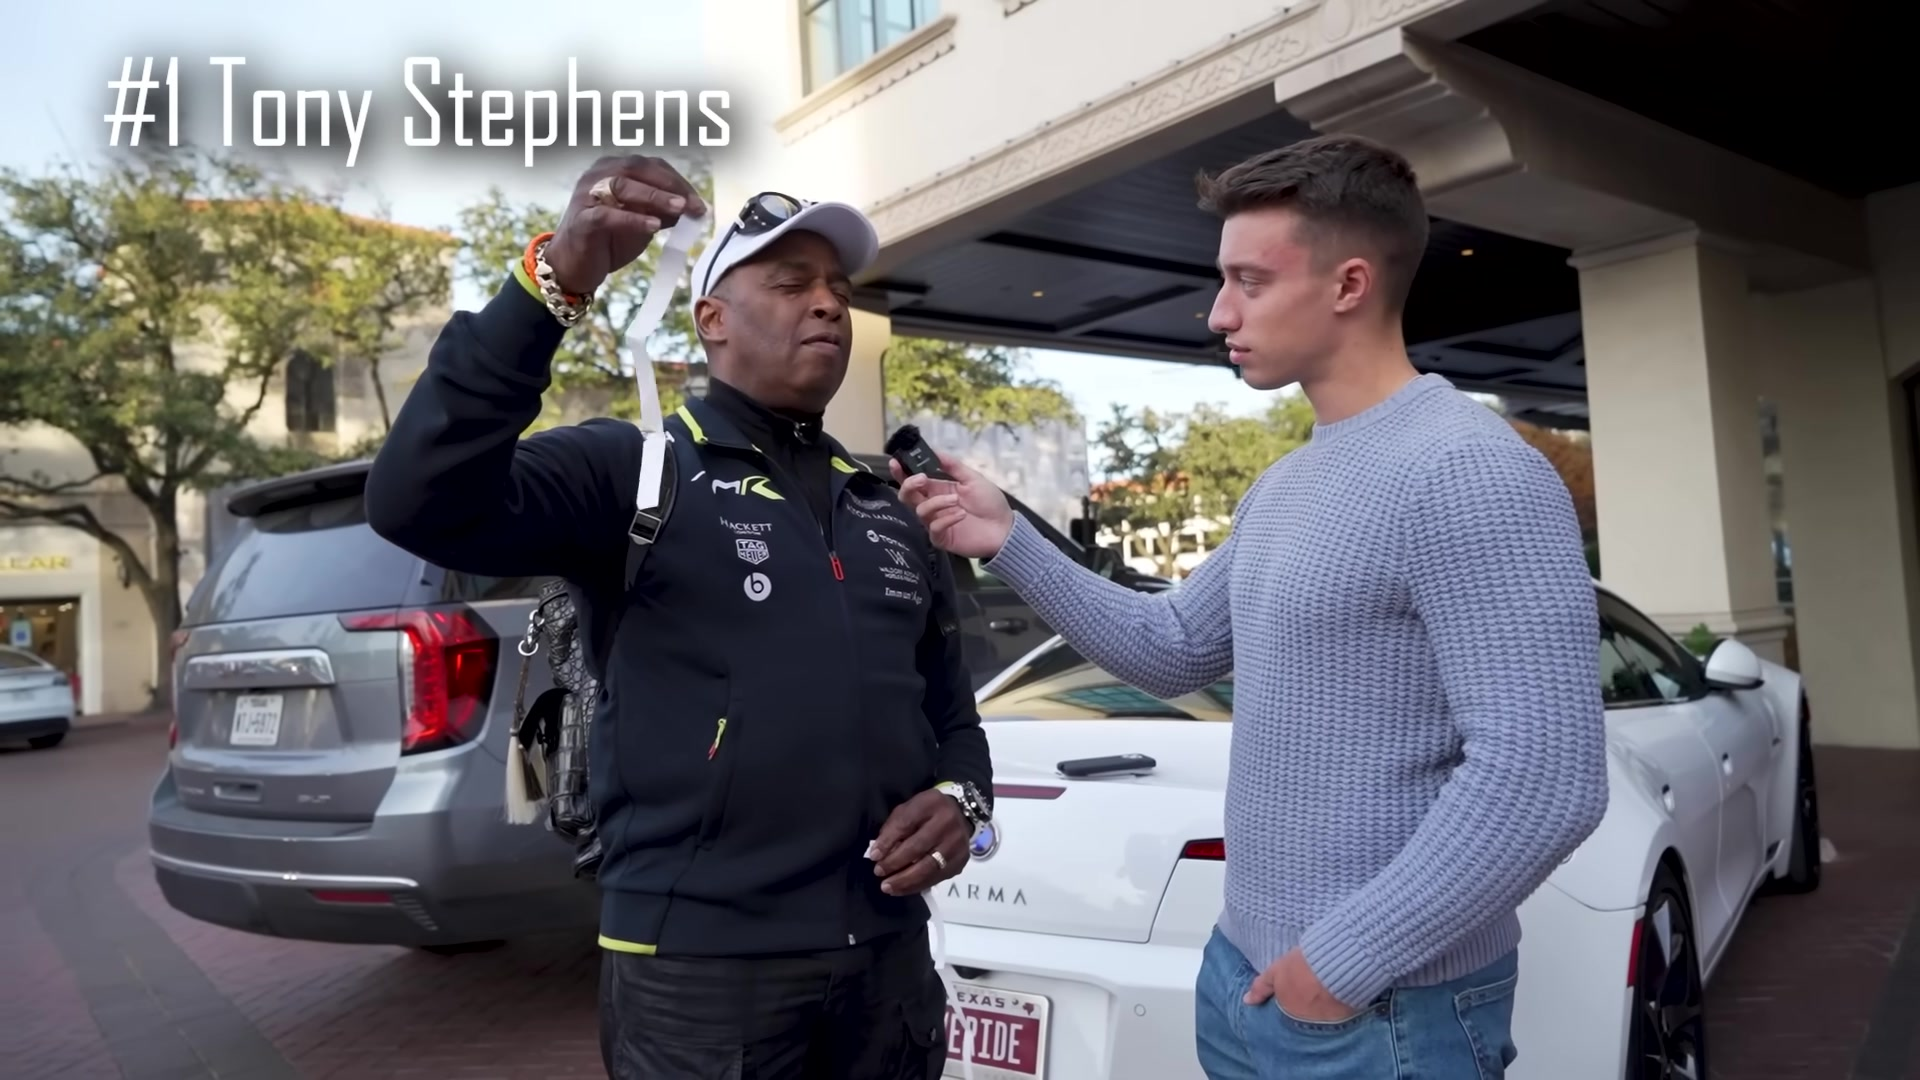
\includegraphics[width=\textwidth]{manuscript/figures/ch01-tony-stephens-ribbon.jpg}
\caption{Tony Stephens holds the paper strip he has torn to represent the
finite portion of life still available. Frame from School of Hard Knocks at
00:22:40.}
\label{fig:remaining-ribbon}
\end{figure}

The exact ages in the demonstration are illustrative and should not be used as
a forecast. Its value is visual. Money compounds because an asset can remain
invested through time. Time itself does not compound for its owner. An hour
cannot be retained this year and spent twice next year. Health affects the
range of uses available within an hour. Attention determines whether the hour
is experienced at all.

We can write a life budget with the same honesty used for a cash budget. Let
$T$ be discretionary hours after sleep, care, necessary work, and basic
maintenance. Let $a_i$ be the hours assigned to activity $i$. Then

\begin{equation}
\sum_i a_i \leq T.
\end{equation}

There is no debt instrument that can relax this constraint. Help can transfer
tasks. Money can buy convenience, care, proximity, and recovery. Systems can
separate income from the owner's next hour. Yet every strategy still spends
someone's time: the owner's, a worker's, a partner's, a family member's, or a
future person's. A serious account of wealth asks whose hours have been saved
and whose have been consumed.

This is where a status definition of rich becomes dangerous. Status has no
natural stopping point. The comparison group changes as soon as the person
enters a wealthier room. A number that once represented safety becomes evidence
of insufficiency. Spending expands to make the new position visible, which
raises $S$, which raises the capital target $P$, which requires more time
from the very life the target was meant to free.

The loop is simple:

\begin{equation}
\begin{aligned}
\text{comparison}
  &\longrightarrow \text{higher fixed spending}\\
  &\longrightarrow \text{higher required capital}\\
  &\longrightarrow \text{more compulsory effort}.
\end{aligned}
\end{equation}

The loop is not broken by pretending desire is shameful. Comfort, beauty,
travel, craft, hospitality, and generous experiences can all enrich a life. It
is broken by making desire answer a concrete question: \emph{What will this add
after its full claim on money, maintenance, attention, and future work?}

\section{Define enough as a set of capabilities}

A useful definition of enough should be demanding enough to guide decisions and
flexible enough to survive a changed life. It needs at least five layers.

First is a \textbf{material floor}: safe shelter, food, healthcare, care
obligations, essential transport, and protection against foreseeable shocks.
Second is a \textbf{freedom floor}: enough margin to refuse work, debt, or a
relationship that violates a serious boundary. Third is a \textbf{time design}:
the hours reserved for health, close relationships, rest, learning, and work
worth doing. Fourth is a \textbf{risk boundary}: the losses that no opportunity
is allowed to impose on the household or on people who did not consent to the
bet. Fifth is a \textbf{surplus purpose}: the people, institutions, places, or
problems that become eligible for attention when consumption no longer needs
the next dollar.

The first two layers establish abundance. Time design and surplus purpose make
fulfillment possible. The risk boundary protects both, while the willingness
to state a sufficient floor makes contentment operational rather than
sentimental.

These layers turn enough from a mood into an operating definition. A reader can
write:

\begin{quote}
\small
I have enough for this stage when ordinary needs are secure, a defined shock
does not force a destructive choice, my essential time is protected, my work
does not violate the people it depends on, and additional accumulation has a
named use.
\end{quote}

The phrase \emph{for this stage} matters. Enough is not an oath never to build
again. A child arrives. A parent needs care. A business enters a capital-heavy
season. A person discovers a problem worth a decade. The definition can change,
but it should change in daylight. Otherwise every expansion of appetite can
masquerade as necessity.

\section{The first wealth statement}

Before choosing an investment, company, or career, write a one-page wealth
statement. It should answer six questions in plain language:

\begin{enumerate}
\item What material insecurity would more money relieve now?
\item What annual life are current assets and skills expected to support?
\item Which freedoms matter enough to protect before status spending?
\item Which people and obligations must survive a failed plan?
\item What amount of time will not be traded away for a larger number?
\item Once the material and freedom floors are secure, what is surplus for?
\end{enumerate}

Do not begin with an impressive target. Begin with the life, then label the
resources that could support it: earned income, portable skills, reserves,
insurance where appropriate, productive assets, community, family agreements,
and work one would still choose if the audience disappeared.

The result will not tell you how to get rich. It will do something prior and
more valuable: it will tell you which forms of getting rich would defeat their
own purpose.

A desired life is not built on desire alone. People begin with unequal health,
money, safety, education, geography, and access. The next chapter turns from the
destination to that starting line, because honest agency begins by seeing the
ground beneath one's feet.
